\documentclass[12pt,a4paper]{article}
\usepackage[utf8]{inputenc}
\usepackage[portuguese]{babel}
\usepackage[T1]{fontenc}
\usepackage{geometry}
\geometry{a4paper, margin=2.5cm}
\usepackage{graphicx}
\usepackage{hyperref}
\usepackage{tabularx}
\usepackage{booktabs}
\usepackage{enumitem}
\usepackage{xcolor}
\usepackage{float}
\usepackage{caption}

\title{\textbf{Atividade 3: Requisitos e Backlog} \\ \large MC656 - Engenharia de Software}
\author{
    Giovanni Santos Scalabrin - RA: 281210 \\
    Rodrigo Banin - RA: 238257 \\
    Leandro Marcos Checchio de Souza - RA: 244784 \\
    Lucca Maso Miranda - RA: 281827
}
\date{\today}

\begin{document}

\maketitle

\section{Elicitação de Requisitos}

\subsection{Técnica Escolhida}
A técnica escolhida foi o \textbf{Benchmarking}. 
Como o sistema \textit{sabrielGoares} visa atender a diferentes cenários institucionais (Centro Acadêmico, Condomínio e Orçamento Participativo), a análise comparativa de plataformas consolidadas no mercado permite identificar as melhores práticas de auditoria e usabilidade, bem como mapear lacunas que nosso sistema precisa preencher (como a unificação de diferentes regras de elegibilidade em um único motor).

\subsection{Fontes Utilizadas}
Foram analisados dois sistemas de código aberto que resolvem partes do escopo do nosso projeto:
\begin{itemize}
    \item \textbf{Helios Voting:} Sistema de votação online com verificação ponta a ponta (E2E), referência em eleições acadêmicas.
    \item \textbf{Decidim:} Plataforma digital para participação cidadã, utilizada no Orçamento Participativo de diversas cidades.
\end{itemize}

\subsection{Condução da Atividade}
A atividade foi conduzida por meio de análise documental, testes empíricos de fluxo de usuário nas plataformas e revisão de suas especificações técnicas disponíveis publicamente. O foco foi em três eixos: Elegibilidade/Pesos, Sigilo/Auditoria e Fluxo de Propostas.

\subsection{Evidências (Comparativo Técnico)}
\begin{table}[H]
\centering
\begin{tabularx}{\textwidth}{>{\hsize=.2\hsize}X >{\hsize=.4\hsize}X >{\hsize=.4\hsize}X}
\toprule
\textbf{Característica} & \textbf{Helios Voting} & \textbf{Nossa Solução (\textit{sabrielGoares})} \\
\midrule
Sigilo & Absoluto (Criptografia Homomórfica) & Configurável por tipo de eleição \\
Pesos de Voto & Igualitário (1 voto = 1 pessoa) & Suporte a pesos proporcionais flexíveis \\
Auditoria & Alta complexidade (cerimônia de chaves) & Auditoria simplificada para leigos \\
\bottomrule
\end{tabularx}
\caption{Comparativo de funcionalidades.}
\end{table}

\subsection{Principais Descobertas e Necessidades}
\begin{itemize}
    \item O \textit{Helios Voting} possui um sistema de auditoria extremamente seguro, mas que gera grande atrito por eleitores leigos devido à complexidade da interface.
    \item Nenhuma das plataformas analisadas lida nativamente com "pesos proporcionais" atrelados a bens (ex: fração ideal em condomínios) no mesmo motor de votação secreta.
    \item No \textit{Decidim}, o processo exige aprovação técnica administrativa antes da proposta ir para votação pública.
\end{itemize}

\section{Da Elicitação aos Requisitos}

\subsection{Matriz de Rastreabilidade}
A tabela abaixo demonstra como as descobertas obtidas deram origem aos requisitos.

\begin{table}[H]
\centering
\begin{tabularx}{\textwidth}{>{\hsize=.35\hsize}X >{\hsize=.35\hsize}X >{\hsize=.3\hsize}X}
\toprule
\textbf{Descoberta da Elicitação} & \textbf{Análise / Interpretação} & \textbf{Requisito Relacionado} \\
\midrule
O fluxo de auditoria do Helios gera abandono de leigos. & A auditoria não pode interromper o fluxo principal. Comprovante deve ser passivo. & RNF - Usabilidade \newline \textbf{Épico:} \href{https://github.com/gsscala/MC656/issues/15}{\#15 - Auditoria} \\
Sistemas analisados não suportam pesos desiguais flexíveis. & É necessário um módulo (\texttt{contextrule}) que calcule o peso antes do depósito na urna. & RF - Cálculo de Peso \newline \textbf{História:} \href{https://github.com/gsscala/MC656/issues/14}{\#14 - Voto com Peso} \\
O Decidim exige moderação prévia. & O sistema precisa de fluxo onde o Admin avalia propostas antes da cédula final. & RF - Validação \newline \textbf{História:} \href{https://github.com/gsscala/MC656/issues/19}{\#19 - Submissão de Proposta} \\
\bottomrule
\end{tabularx}
\end{table}

\subsection{Requisitos Não Funcionais Relevantes}
\begin{itemize}
    \item \textbf{Usabilidade:} O fluxo de votação deve ser concluído em no máximo 3 cliques por eleitores com baixa afinidade tecnológica.
    \item \textbf{Desempenho:} O registro do voto não deve exceder 2 segundos para evitar cliques duplos.
\end{itemize}

\section{Épicos, Histórias e Critérios de Aceitação}

\subsubsection*{Épico \href{https://github.com/gsscala/MC656/issues/12}{\#12 - Motor de Votação e Cédulas}}
\textbf{História \href{https://github.com/gsscala/MC656/issues/13}{\#13} - Registro de Voto Simples (Centro Acadêmico)}
\begin{itemize}
    \item \textbf{Descrição:} Como eleitor de lista fechada, quero selecionar uma chapa e confirmar meu voto, para registrar minha escolha com sigilo.
    \item \textbf{Critérios de Aceitação:}
    \begin{itemize}
        \item O sistema deve exibir apenas chapas/opções ativas para a eleição.
        \item Ao confirmar, o voto deve ser salvo no banco de dados sem associar a identidade (user\_id) ao payload da cédula.
        \item O usuário deve ser redirecionado para uma tela de sucesso após o envio.
    \end{itemize}
\end{itemize}

\textbf{História \href{https://github.com/gsscala/MC656/issues/14}{\#14} - Votação com Peso Proporcional (Condomínio)}
\begin{itemize}
    \item \textbf{Descrição:} Como condômino, quero que meu voto seja multiplicado pela minha fração ideal, para que a apuração seja justa e siga a convenção do condomínio.
    \item \textbf{Critérios de Aceitação:}
    \begin{itemize}
        \item O sistema deve recuperar a fração ideal do eleitor no momento da geração da cédula.
        \item O payload do voto salvo na urna deve conter o multiplicador de peso.
    \end{itemize}
\end{itemize}

\subsubsection*{Épico \href{https://github.com/gsscala/MC656/issues/15}{\#15 - Auditoria e Comprovantes}}
\textbf{História \href{https://github.com/gsscala/MC656/issues/16}{\#16} - Geração de Recibo de Voto}
\begin{itemize}
    \item \textbf{Descrição:} Como eleitor, quero receber um código de recibo após votar, para poder auditar futuramente que meu voto foi depositado na urna corretamente.
    \item \textbf{Critérios de Aceitação:}
    \begin{itemize}
        \item O sistema deve gerar um hash único (ex: SHA-256) baseado nos dados da cédula e carimbo de tempo.
        \item O hash deve ser exibido na tela final de sucesso para o eleitor copiar/salvar.
    \end{itemize}
\end{itemize}

\textbf{História \href{https://github.com/gsscala/MC656/issues/17}{\#17} - Verificação de Apuração Pública}
\begin{itemize}
    \item \textbf{Descrição:} Como auditor independente, quero acessar a lista de hashes e votos anonimizados, para atestar que a urna não foi violada e o resultado está correto.
    \item \textbf{Critérios de Aceitação:}
    \begin{itemize}
        \item Deve existir uma rota pública (se configurado) que retorne a lista de votos (apenas payload e hash).
        \item O auditor deve conseguir re-calcular o resultado da eleição somando os pesos da lista pública.
    \end{itemize}
\end{itemize}

\subsubsection*{Épico \href{https://github.com/gsscala/MC656/issues/18}{\#18 - Propostas e Elegibilidade}}
\textbf{História \href{https://github.com/gsscala/MC656/issues/19}{\#19} - Submissão de Proposta Técnica (Orçamento Participativo)}
\begin{itemize}
    \item \textbf{Descrição:} Como cidadão, quero enviar uma proposta de obra pelo sistema, para que seja avaliada e, se aprovada, incluída na cédula de votação do orçamento municipal.
    \item \textbf{Critérios de Aceitação:}
    \begin{itemize}
        \item Formulário contendo título, descrição detalhada e orçamento estimado.
        \item Ao enviar, a proposta entra automaticamente no status "Pendente de Análise Técnica".
    \end{itemize}
\end{itemize}

\textbf{História \href{https://github.com/gsscala/MC656/issues/20}{\#20} - Controle de Quórum Mínimo}
\begin{itemize}
    \item \textbf{Descrição:} Como administrador de uma assembleia, quero definir um quórum mínimo de participação, para que a eleição tenha validade legal.
    \item \textbf{Critérios de Aceitação:}
    \begin{itemize}
        \item A tela de criação de eleição deve ter um campo opcional numérico para "Quórum Mínimo".
        \item A apuração oficial só deve ser considerada "Concluída com Validade" se a soma de participação atingir o quórum.
    \end{itemize}
\end{itemize}


\section{Organização e Priorização do Backlog}

A partir desta etapa, o backlog do projeto foi orientado a valor, visando entregar primeiro as funcionalidades fundamentais de um sistema de votação seguro.

\subsection{Priorização de Épicos}
\begin{table}[H]
\centering
\begin{tabularx}{\textwidth}{c c c X}
\toprule
\textbf{Prioridade} & \textbf{Épico} & \textbf{1ª Entrega?} & \textbf{Justificativa} \\
\midrule
1 & \href{https://github.com/gsscala/MC656/issues/12}{\#12 - Motor de Votação} & Sim & É o núcleo do sistema. Sem o depósito correto de cédulas, as demais funcionalidades não têm valor prático. \\
2 & \href{https://github.com/gsscala/MC656/issues/15}{\#15 - Auditoria} & Sim & É o diferencial competitivo do sistema. Garantir recibos e transparência é essencial para a confiança institucional desde o dia zero. \\
3 & \href{https://github.com/gsscala/MC656/issues/18}{\#18 - Propostas} & Não & O gerenciamento de propostas (Orçamento Participativo) pode ser adicionado numa segunda iteração. O foco inicial deve ser validar o motor de urna. \\
\bottomrule
\end{tabularx}
\end{table}

\subsection{Priorização das Histórias por Épico}
A primeira entrega de valor é composta pelo motor básico de votação e geração de recibos. As tabelas a seguir detalham a priorização das histórias dentro de cada épico.

\subsubsection*{Épico \href{https://github.com/gsscala/MC656/issues/12}{\#12 - Motor de Votação e Cédulas}}
\begin{table}[H]
\centering
\begin{tabularx}{\textwidth}{c c c X}
\toprule
\textbf{Prioridade} & \textbf{História} & \textbf{1ª Entrega?} & \textbf{Justificativa} \\
\midrule
1 & \href{https://github.com/gsscala/MC656/issues/13}{\#13 - Voto Simples} & Sim & Caminho feliz e requisito fundamental para que ocorra uma eleição. \\
2 & \href{https://github.com/gsscala/MC656/issues/14}{\#14 - Voto com Peso} & Não & Adiciona complexidade lógica inicial desnecessária para provar a viabilidade da arquitetura da urna. \\
\bottomrule
\end{tabularx}
\caption{Priorização das histórias do Épico \#12 - Motor de Votação e Cédulas.}
\end{table}

\subsubsection*{Épico \href{https://github.com/gsscala/MC656/issues/15}{\#15 - Auditoria e Comprovantes}}
\begin{table}[H]
\centering
\begin{tabularx}{\textwidth}{c c c X}
\toprule
\textbf{Prioridade} & \textbf{História} & \textbf{1ª Entrega?} & \textbf{Justificativa} \\
\midrule
1 & \href{https://github.com/gsscala/MC656/issues/16}{\#16 - Recibo de Voto} & Sim & Mitiga o risco de desconfiança do eleitor assim que o voto é depositado. \\
2 & \href{https://github.com/gsscala/MC656/issues/17}{\#17 - Verificação Pública} & Não & A auditoria individual (recibo) é mais prioritária que a auditoria global inicial. \\
\bottomrule
\end{tabularx}
\caption{Priorização das histórias do Épico \#15 - Auditoria e Comprovantes.}
\end{table}

\subsubsection*{Épico \href{https://github.com/gsscala/MC656/issues/18}{\#18 - Propostas e Elegibilidade}}
\begin{table}[H]
\centering
\begin{tabularx}{\textwidth}{c c c X}
\toprule
\textbf{Prioridade} & \textbf{História} & \textbf{1ª Entrega?} & \textbf{Justificativa} \\
\midrule
1 & \href{https://github.com/gsscala/MC656/issues/19}{\#19 - Submissão de Proposta} & Não & É pré-requisito lógico para o quórum: sem propostas aprovadas na cédula, o controle de participação mínima não tem utilidade prática. \\
2 & \href{https://github.com/gsscala/MC656/issues/20}{\#20 - Controle de Quórum} & Não & Depende da existência de propostas e de uma eleição já funcional. Agrega valor ao validar legalmente a votação, mas só faz sentido após o fluxo básico de propostas. \\
\bottomrule
\end{tabularx}
\caption{Priorização das histórias do Épico \#18 - Propostas e Elegibilidade.}
\end{table}

\subsection{Priorização Global das Histórias}
A tabela abaixo consolida a priorização de todas as histórias do projeto em ordem global, evidenciando as prioridades relativas entre histórias de épicos distintos.

\begin{table}[H]
\centering
\begin{tabularx}{\textwidth}{c c c X}
\toprule
\textbf{Prioridade} & \textbf{História} & \textbf{1ª Entrega?} & \textbf{Justificativa} \\
\midrule
1 & \href{https://github.com/gsscala/MC656/issues/13}{\#13 - Voto Simples} & Sim & Caminho feliz e requisito fundamental para que ocorra uma eleição. \\
2 & \href{https://github.com/gsscala/MC656/issues/16}{\#16 - Recibo de Voto} & Sim & Mitiga o risco de desconfiança do eleitor assim que o voto é depositado. \\
3 & \href{https://github.com/gsscala/MC656/issues/14}{\#14 - Voto com Peso} & Não & Adiciona complexidade lógica inicial desnecessária para provar a viabilidade da arquitetura da urna. \\
4 & \href{https://github.com/gsscala/MC656/issues/17}{\#17 - Verificação Pública} & Não & A auditoria individual (recibo) é mais prioritária que a auditoria global inicial. \\
5 & \href{https://github.com/gsscala/MC656/issues/19}{\#19 - Submissão de Proposta} & Não & É pré-requisito lógico para o quórum, mas depende de um motor de votação já funcional. \\
6 & \href{https://github.com/gsscala/MC656/issues/20}{\#20 - Controle de Quórum} & Não & Depende da existência de propostas e de uma eleição já funcional. Agrega valor ao validar legalmente a votação, mas só faz sentido após o fluxo básico de propostas. \\
\bottomrule
\end{tabularx}
\caption{Priorização global de todas as histórias do projeto.}
\end{table}

\subsection{Snapshot do GitHub Projects}
A organização do backlog orientada a valor foi realizada utilizando a ferramenta GitHub Projects.

\vspace{1cm}
\begin{center}
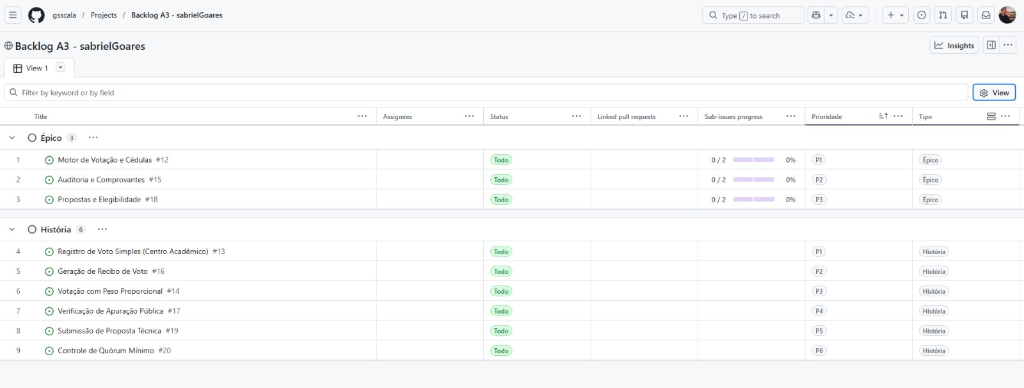
\includegraphics[width=\textwidth]{board.png}
\captionof{figure}{Organização do Backlog no GitHub Projects.}
\end{center}

\end{document}
